    \chapter{Estado del Arte}
    \section{Software a desarrollar}
    \subsection{Aplicaciones de aprendizaje}
    Actualmente existen numerosas aplicaciones que ayudan a la adquisición de conocimientos sobre distintos temas, 
    como los idiomas, las matemáticas o la teoría para la conducción de un vehículo, entre otros. A continuación se
    detallarán las aplicaciones más destacadas encontradas en el mercado
   
    \subsubsection{Duolingo}
    \begin{wrapfigure}{r}{0.25\textwidth}
        \vspace*{-0.4cm}

        \centering
        
\includegraphics[width=0.2\textwidth]{imagenes/c2/duolingo.png}
        \caption{Logo de Duolingo}
        \vspace*{-0.15cm}
    \end{wrapfigure}

    Duolingo es una de las aplicaciones más populares que existen para aprender idiomas. Esta aplicación se basa en el método
    de aprendizaje por inmersión, en el que el usuario estudia el idioma mediante una serie de actividades lúdicas.
    La aplicación se divide en lecciones o temas, las cuales contienen una serie de ejercicios que el usuario debe
    completar para ir avanzando por las distintas secciones. Estos ejercicios son muy variados y consisten en, por ejemplo,
    la traducción de palabras o frases con el teclado, la traducción de estas seleccionando bloques de palabras, la
    pronunciación de palabras o frases mediante el micrófono del dispositivo, la selección de imágenes, etc. Además,
    Duolingo ofrece en cada lección, antes de cada ejercicio, una breve explicación de la gramática o vocabulario con
    imágenes y explicaciones sencillas. Esta aplicación es gratuita (aunque tiene mejoras de pago dentro de esta) 
    y está disponible para dispositivos móviles (Android, iOS y Windows Phone).
 

    \subsubsection{Artly}
    Artly es una aplicación móvil que permite aprender cientas de obras de arte de forma interactiva. Cuando el usuario abre la app, 
    se encuentra una lista intuitiva de secciones de los distintos movimientos artísticos, los cuales se irán desbloqueando uno a uno
    conforme el usuario vaya completado las lecciones de cada sección. 

    En cada uno de los apartados el usuario podrá ver una lista de cuadros y esculturas de los distintos artistas que pertenecen a ese movimiento.
    Al seleccionar uno de ellos, se abrirá una pantalla con la imagen del cuadro o escultura, en la que el usuario podrá ver la obra más de cerca, junto
    con el título, la persona autora y una descripción. 
    Tras esto, el usuario puede seleccionar el botón de "Inicar Lección" para acceder a una serie de preguntas sobre las obras vistas en dicho apartado (seleccionar el autor, seleccionar el título de la obra...). 
    Al finalizar las preguntas, el usuario sumará un progreso en el tema que permitirá desbloquear otros apartados y conseguir ciertos logros en su perfil.
    La aplicación es gratuita pero tiene mejoras de pago que te permitirán avanzar con más facilidad y sin anuncios.

    \begin{figure}[H]

        \centering
        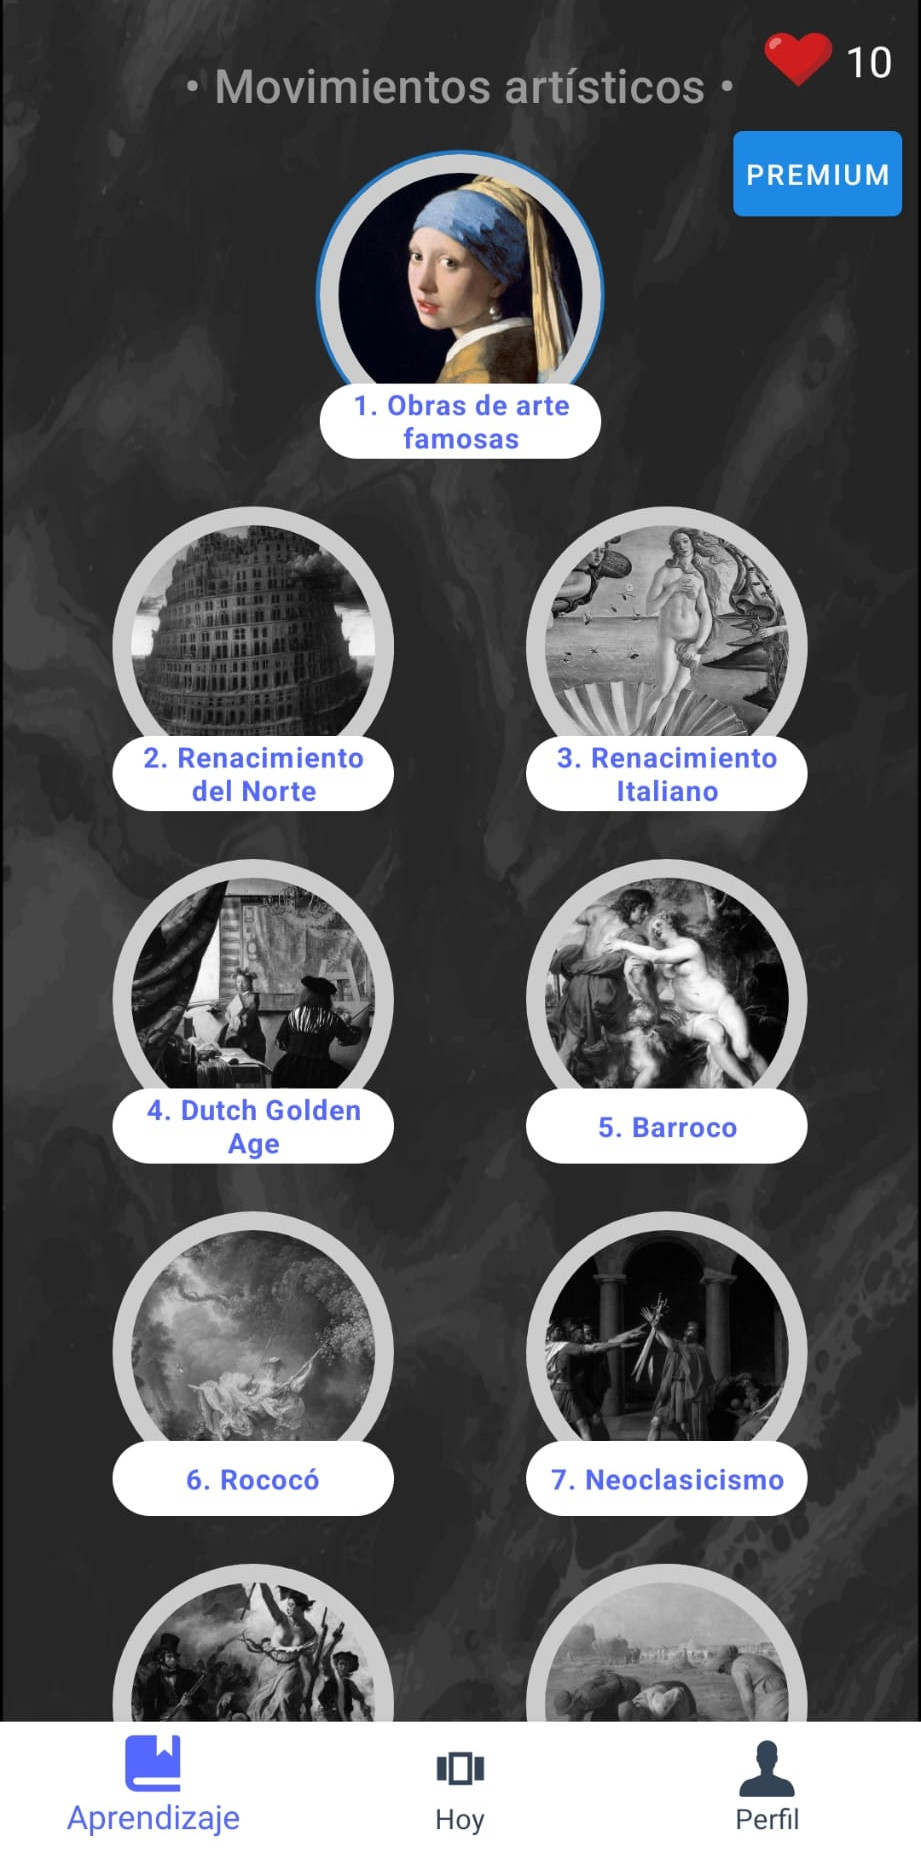
\includegraphics[width=0.4\textwidth]{imagenes/c2/artly.jpeg}
        \caption{Vista del menú de secciones de Artly}
    \end{figure}


    
    \subsubsection{BMath}
    BMath es un software para móviles para el aprendizaje de conceptos matemáticos mediante gamificación. Esta aplicación crea un programa personalizado para el
    usuario en función del curso académico en el que esté, adaptándose a su conocimiento y a su nivel. Pese a ser gratuita, el tiempo diario que te permite el
    modo gratutito es de 5 mintuos, mientras que si pagas te permitirá ampliarlo en 10 minutos cada día. 

    Es un ejemplo de aprendizaje por gamificación ya que la aplicación es prácticamente un videojuego, pues muestra una ciudad por la que te puedes mover y donde construyes distintos edificios. Para construirlos, deberás superar
    una serie de pruebas sobre álgebra, geometría, etc. También obtendrás puntos de experiencia al superar los ejercicios y, al subir de nivel, obtendrás nuevos edificios y decoraciones para tu ciudad. Con esto, se pretende que el usuario
    tenga la motivación de realizar ejercicios y superarlos correctamente para lograr que su ciudad prospere. Como alumno también puedes elegir tu propio personaje animado que te identificará en el juego.

    Los diseños del software están muy cuidados y posee colores muy llamativos para que el usuario se sienta motivado y atraido y proporciona una experiencia de usuario agradable y motivadora, ayudando al alumno en todo momento 
    a solucionar los ejercicios y enseñándole técnicas para resolverlos.

    La aplicación también posee otras funciones como un apartado donde añadir recordatorios para acceder a la aplicación, preguntas para conocer cómo se siente el usuario tras cada sesión de estudio, etc.

    \begin{figure}[H]
        \centering
        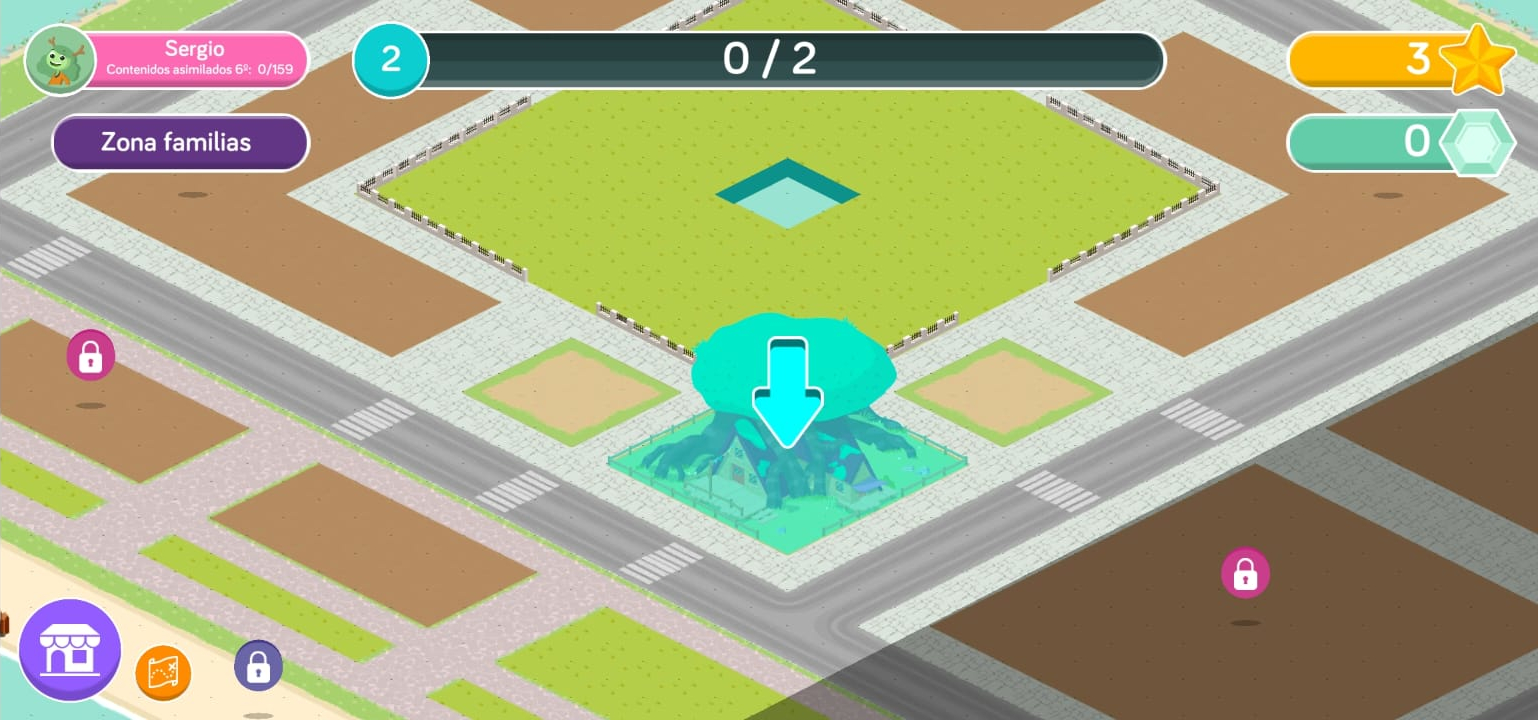
\includegraphics[width=\textwidth]{imagenes/c2/bmath.jpeg}
        \caption{Vista de la ciudad de BMath}
    \end{figure}


    % \subsubsection{FisicaMaster \& QuímicaMaster}

    % \subsubsection{Academons}

    \subsection{Aplicaciones de aprendizaje musical}
    Centrándonos ya en el tema que nos ocupa (el aprendizaje musical) existen numerosas aplicaciones que ayudan a la adquisición
    de conocimientos musicales o a la ayuda a aprender a tocar un instrumento musical. Algunas de estas aplicaciones son:

    \subsubsection{Curso de Lenguaje Musical}
    Esta herramienta para móvil tiene el objetivo de enseñar los conceptos básicos de lenguaje musical. La aplicación proporciona una forma de aprendizaje muy 
    tradicional y que no está basada en la gamificación, ya que no dispone de ningún tipo de seguimiento del progreso ni de ejercicios para realizar sobre las lecciones aprendidas.
    Al abrir la app, aparece una lista de lecciones en las que cuando se seleccione una de ellas, mostrará un vídeo de un profesor explicando el contenido del temario. 

    \subsubsection{Sonid}
    Sonid consiste en una aplicación para el aprendizaje de piano a través de la gamificación.
    La aplicación se divide en distintas lecciones que el usuario irá desbloqueando al pasarlas correctamente.
    Cada lección explica unos conceptos básicos de música y piano y, al finalizar, el usuario deberá realizar una serie
    de ejercicios para comprobar que ha entendido y aprendido el contenido del temario.

    Algunos de los ejercicios que posee esta aplicación son:
    \begin{itemize}
        \item Seleccionar la tecla en el piano que corresponde a una nota musical
        \item Responder si la tecla que se ha pulsado es una nota musical o no
        \item Decidir qué nota musical corresponde a una tecla del piano que se ha pulsado
        \item Etc 
    \end{itemize}

    Además de las lecciones, el usuario también puede practicar con escalas y acordes del piano además de aprenderlas en la wiki y en el diccionario que 
    posee la aplicación. También tiene un foro para que toda la gente pueda compartir sus dudas.

    Por último, en cuanto al seguimiento, el usuario puede ver su progreso y sus estadísticas en su perfil, donde aparece el número de lecciones
    completadas, el número de errores que ha tenido, la experiencia que tiene. Además, el usuario consigue logros al completar las lecciones y 
    comparte una clasificación global con otros usuarios que también usan la aplicación.

    \subsubsection{--}

  



    \section{Desarrollo de Software}
\subsection{Flutter}
\begin{wrapfigure}{r}{0.27\textwidth}
    \vspace*{-0.4cm}
    \centering
    
\includegraphics[width=0.27\textwidth]{imagenes/c2/flutter.png}
    
    \caption{Logo de Flutter}
\end{wrapfigure}Flutter es un kit de desarrollo software de código abierto destinado al desarrollo de aplicaciones móviles. Está programado en Dart y fue creado por Google.
Suele ser usado para realizar aplicaciones para móvil, web y escritorio desde una sola base de código, lo cual permite mucha más agilidad y consistencia.

Flutter ofrece tres ventajas respecto a otros frameworks utilizados para el desarrollo de aplicaciones multiplataformas:

\begin{itemize}
    \item \textbf{Compilación en nativo}
    \item \textbf{Flexibilidad} para crear interfaces gráficas
    \item \textbf{Desarrollo veloz}, permitiendo ver el resultado del código al instante.

\end{itemize}
Flutter está basado en el concepto de widgets, los cuales son elementos gráficos que componen la vista. 

\subsection{React Native}
Framework de código abierto creado por Meta Platforms y destinado al desarrollo de aplicaciones Android, iOS, Web, Windows...
Está basado en Javascript y React y permite crear aplicaciones nativas multiplataforma.


\subsection{Dart}
\subsection{Kotlin}

\subsection{NodeJS}

\subsection{React}
\subsection{Angular}
\subsection{SQL}